% Created 2020-02-04 Tue 10:17
% Intended LaTeX compiler: pdflatex
\documentclass[t]{beamer}
                \usepackage[orientation=portrait,size=a0,scale=1.2,debug]{beamerposter}
                \usepackage[absolute,overlay]{textpos}
                \usepackage{tikz}
                \usepackage{pgfplots}
                \usetikzlibrary{arrows}
                                \usepackage[backend=biber, maxbibnames=2, maxcitenames=2, sortcites=true, style=authoryear]{biblatex}
\AtEveryBibitem{%
\clearfield{issn} % Remove issn
\clearfield{doi} % Remove doi
\ifentrytype{online}{}{% Remove url except for @online
\clearfield{url}
}
}
\renewcommand*{\bibfont}{\small}
\usepackage{./beamerthemedonders}
\usepackage[T1]{fontenc}
\usepackage[utf8]{inputenc}
\usepackage{microtype}
\author{
Daniel Guimarães
\\
\vspace{5mm}
\normalsize{European Masters of Computational Logic - }
\normalsize{(TU Dresden, FU Bozen and TU Wien)}
}
\usetheme{default}
\useinnertheme{rectangles}
\date{\today}
\title{Performance of Survival Models on Predictive Maintenance of Construction Machines}
\hypersetup{
 pdfauthor={Daniel Guimaraes},
 pdftitle={Performance of Survival Models on Predictive Maintenance of Construction Machines},
 pdfkeywords={},
 pdfsubject={},
 pdfcreator={Emacs 27.0.50 (Org mode 9.1.9)}, 
 pdflang={English}}
\begin{document}


\begin{frame}[label={sec:orgc2b2963}]{}
\begin{columns}
\begin{column}{0.3\columnwidth}
\begin{block}{Context}
Manufacturers of construction machines nowadays often provide tools to contractors 
to monitor through a telecommunication device the state of machines. Besides 
telematics data, repair information are sometimes collected by mechanics with 
the intention of improving the mainenance strategy. These two sources of data 
allow the construction of statistical models capable of condition-based 
maintenance. This study demonstrates the process of building, testing and 
validating the survival predictive models in the context of 
construction machines. 

There are normally two parties involved in the repair of machines, the 
construction contractor who outsources the repair service to the repair provider, 
which supply the necessary service, mechanics and tools in turn.

A repair, identified by a Scheinnummer, consists of multiple interventions in a single machine.
\begin{figure}[htbp]
\centering
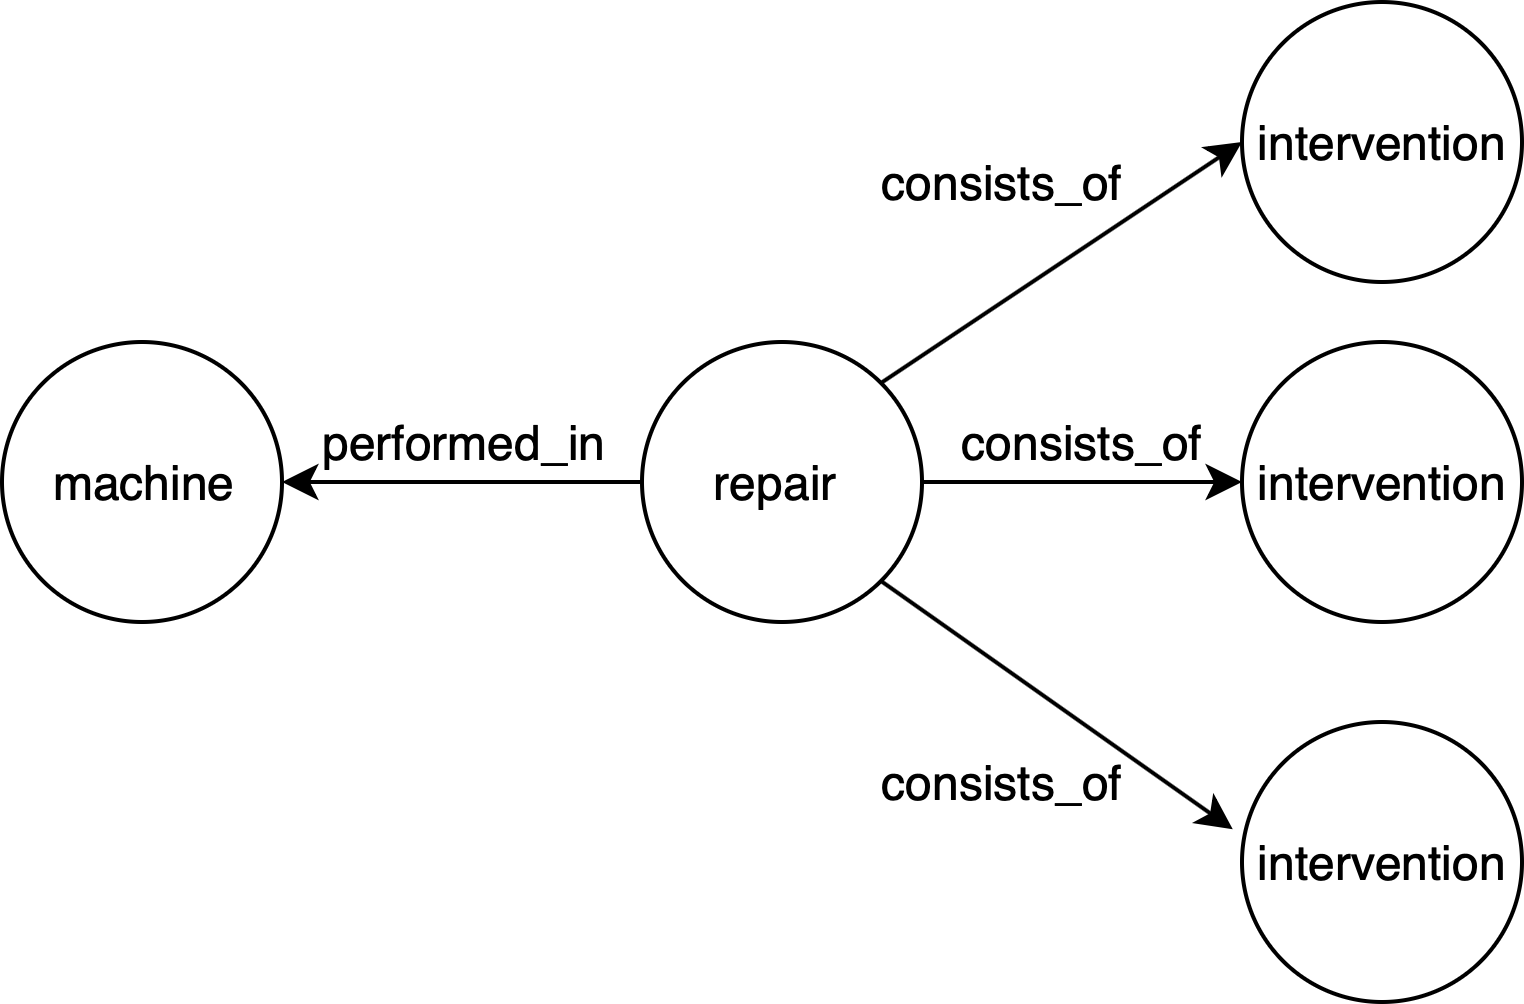
\includegraphics[width=.9\linewidth]{./Logos/repair_schema.png}
\caption{\label{fig:org2f136f4}
Repair overview}
\end{figure}
An intervention, identified by a Scheinnummer and a Zeilennummer, is a part of a repair which occur in a component of a machine.
\begin{figure}[htbp]
\centering
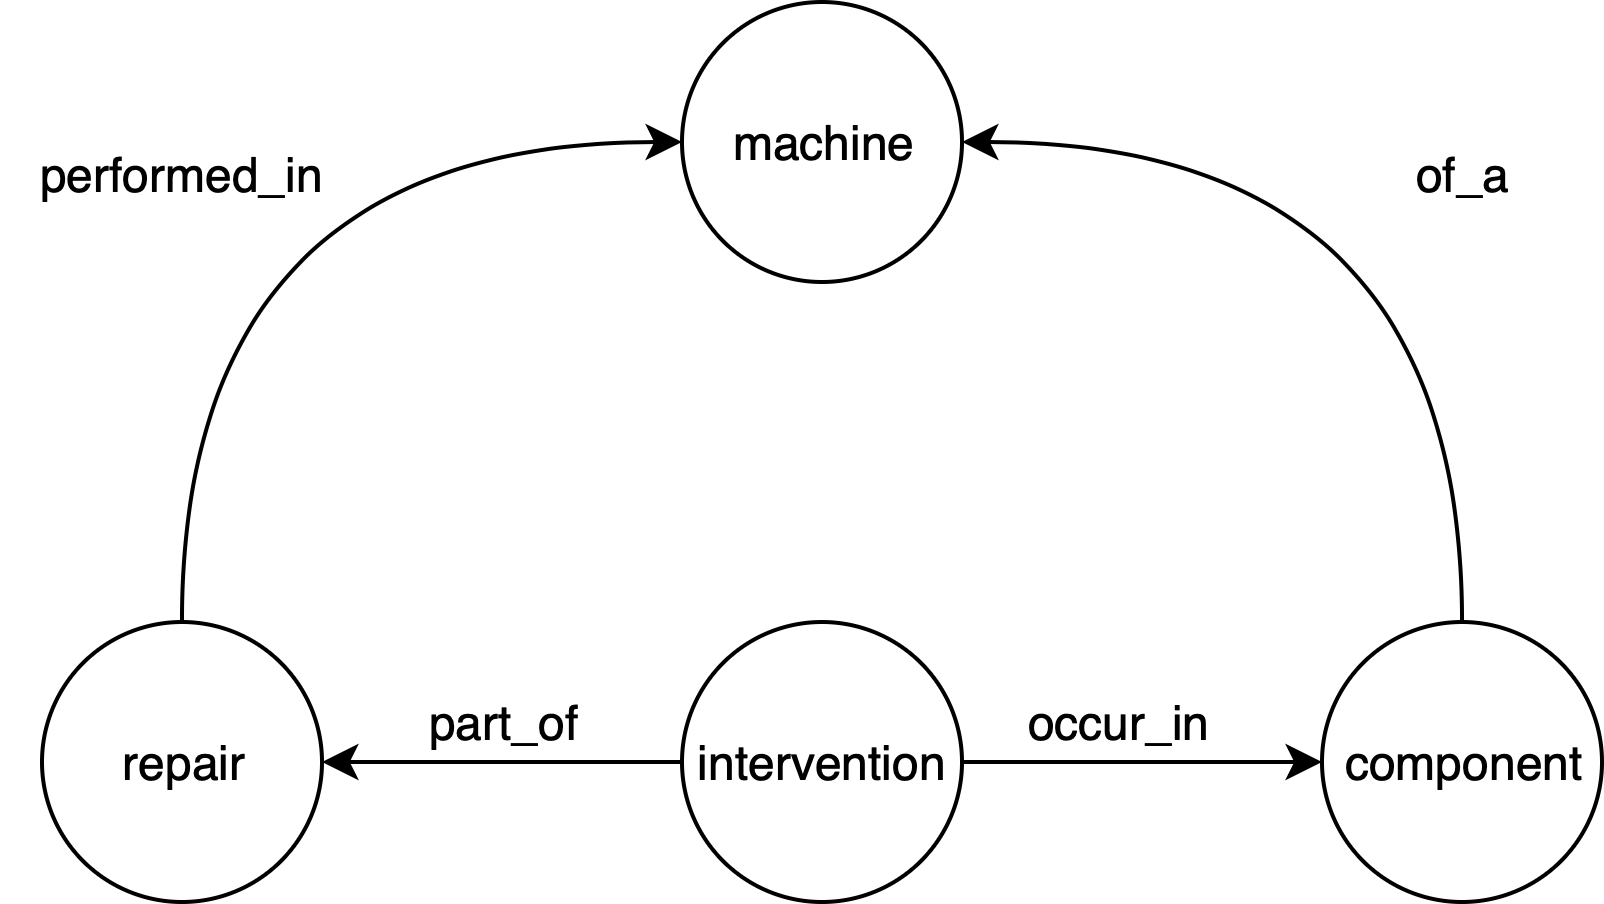
\includegraphics[width=.9\linewidth]{./Logos/intervention_schema.png}
\caption{\label{fig:orge70631a}
Intervention overview}
\end{figure}
 In this study, the main concern is to predict failure events in specific components of
construction machines. Failure events are, however, not directly provided but can
be implied by an specific type of repair, repair-after-failure. In fact, there are two qualities of repair:
\begin{itemize}
\item \alert{Instandsetzung} reactive repair after breakdown preventing the machine from operating, e.g. replacing the motor.
\item \alert{Instandhaltung} a routine maintenance, normally a check, verification; or a minor intervention e.g. changing oil or lubrication.
\end{itemize}
Optimally, from Instandsetzung repairs it is possible to identify failure events, 
those events, in turn, can be used to build a statistical model suitable 
to predict when a failure will occur.
\end{block}

\begin{block}{Relevance}
Despite being used in industrial contexts, the bulk of the scientific work produced on surivival models
are on the medical field. Concerning construction machines, few studies using telematics data. 
Two studies found on this setting were done by Said and Nicoletti\(^{1}\), 
one of them with the collaboration of Perez-Hernandez\(^{2}\). Nevertheless, no 
studies were found on these three criteria: 
on construction machines, using telematics data and with small sample size.
Therefore, the relevance of this work is mostly due to its application and to the 
interesting setting it finds itself.
\end{block}
\end{column}

\begin{column}{0.3\columnwidth}
\begin{block}{Main Questions}
Besides the ultimate question of whether a predictive maintenance model could be generated and used in production.
Other questions had to be answered beforehand, e.g. as mentioned previously, the failure time itself is not known a priori, 
only the time of repair, how is it then possible to predict the time of failure instead of the time of repair?

Additionally, the data was partially collected by humans and hence, susceptible to mistakes. What are the errors captured in the data? 
How to test the sanity of the data? What compromises could be made? Is it possible to improve the quality or "clean" the data?

Telematics data is the most reliable data source, it recorded 18 Paver machines. Under this scarce setting, what is the optimal number of parameters
that could be estimated for the multiparametric model? What mechanisms could be used to deal with scarse data? How to maximize the amount of
data used in the model, i.e. which interventions ocurred in all 18 machines?

Once the model is provided, how reliable is the given model? Is it possible to calculate a residual to measure how far the model is to an
ideal prediction model? Is this model suitable to be put in production?
\end{block}
\begin{block}{Methodology}
The two most primary measures, to calculate the risk of failing is the hazard and survival function.
The survival function gives the probability a machine's life exceed a given time \(x\).
$$ S(t) = P(T\ge x)$$
The survival function has a particular form, for very small values of \(x\), there is a high
probability of surviving over \(x\); as \(x\) grows, this probability decreases, vide:
\begin{figure}[htbp]
\centering
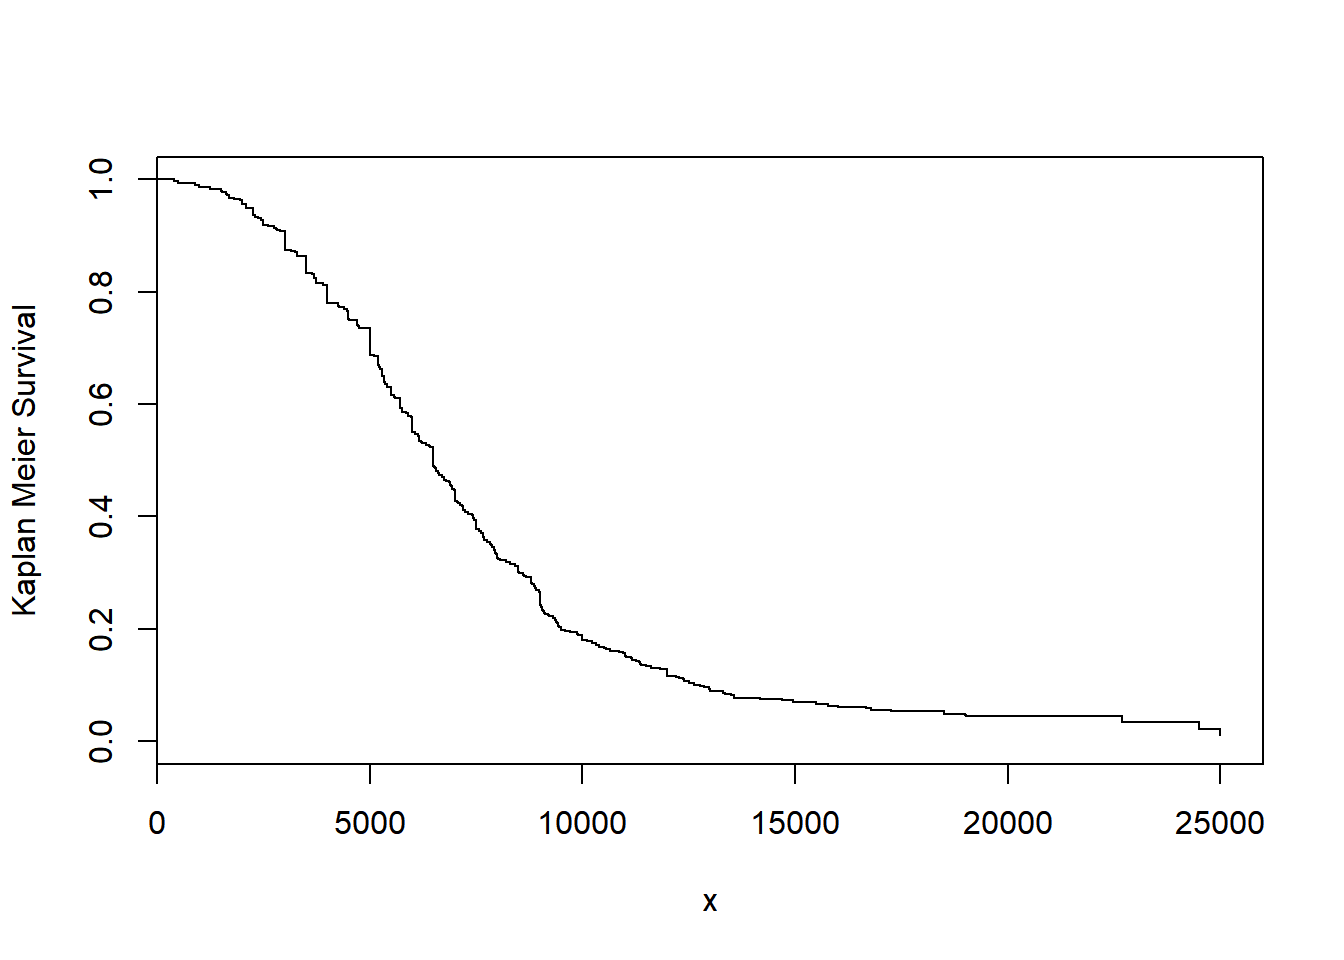
\includegraphics[width=.9\linewidth]{./Logos/survival.png}
\caption{\label{fig:org1ff06fd}
Survival function shape}
\end{figure}

The survival probability of one particular individual can be calculated by using covariates
which influence the failure event, e.g. when predicting a heart attack, whether the patient smokes or his age may be good predictors. 

A prediction model is built by limiting the observation of the covariates until a specific point 
in time often refferred as \alert{cutoff} point. The covariate values in this point
can then used to form a prediction model, yielding the hazard and survival functions
for time points unseen, after the cutoff.

\begin{figure}[H]
    \begin{center}
    \begin{tikzpicture}[thick,scale=3.5]
       % Draw axes
       \draw [->,thick](0,2.5) node (yaxis) [above] {}
	   |- (5,0) node (xaxis) [right] {$time$};
       % Draw two intersecting lines
       \draw[->, thick] (2.5,0.5) coordinate (y_1) --  (4.5,0.5) coordinate (y_2);
       \draw[->, thick] (0,1.0) coordinate (x_1) -- (2.5,1.0) coordinate (x_2);
       \draw [->,thick] (1,1.5) coordinate (d_1) -- (4,1.5) coordinate (d_2);
       \draw [->, thick](2,2.0) coordinate (c_1) -- (3,2.0) coordinate (c_2);
       
       \fill[black] (x_1) circle (1.2pt);
       \fill[black] (c_1) circle (1.2pt);
       \fill[black] (d_1) circle (1.2pt);
       \fill[black] (y_1) circle (1.2pt);
   \end{tikzpicture}
   \qquad % <----------------- SPACE BETWEEN PICTURES
   \begin{tikzpicture}[thick,scale=3.5]
       % Draw axes
       \draw [->,thick](0,2.5) node (yaxis) [above] {}
	   |- (5,0) node (xaxis) [right] {$time$};
       % Draw two intersecting lines
       \draw[dashed] (0,0.5) coordinate (y_1) --  (.8,0.5) coordinate (y_2);
       \draw[dashed] (0,1.0) coordinate (x_1) -- (.8,1.0) coordinate (x_2);
       \draw [dashed] (0,1.5) coordinate (d_1) -- (.8,1.5) coordinate (d_2);
       \draw [dashed](0,2.0) coordinate (c_1) -- (.8,2.0) coordinate (c_2);
       
       \draw[->, thick] (0.8,0.5) coordinate (y_1) --  (2.0,0.5) coordinate (y_2);
       \draw[->, thick] (0.8,1.0) coordinate (x_1) -- (2.5,1.0) coordinate (x_2);
       \draw [->,thick] (0.8,1.5) coordinate (d_1) -- (3,1.5) coordinate (d_2);
       \draw [->, thick](0.8,2.0) coordinate (c_1) -- (1,2.0) coordinate (c_2);
       \draw [dashed](0.8,0) coordinate (p_1) -- (.8,2.5) coordinate (p_2);
       
       \draw[dashed]  (xaxis -| p_2) node[below] {$cutoff$};
   \end{tikzpicture}
   \caption{Selection of the cutoff over subject's follow-up time}
    \label{fig:cutoff}
\end{center}
\end{figure}
\end{block}
\end{column}

\begin{column}{0.3\columnwidth}
\begin{block}{Methodology}
Another concern during this work was how to evaluate the quality of the survival function. Indeed,
validation plays a big part when a model is considered to be put in production. A common validation method
is to calculate the residual between the optimal survival curve, and
the actual. If the survival curve is perfectly able to tell when an failure event will happend
then it will be simply a step function which drops from 1 to 0 when an event happens. This technique, in
the context of survival analysis, is referred as the Brier score, and allows one to evaluate the predictive 
power of the survival function.
\begin{figure}[htbp]
\centering
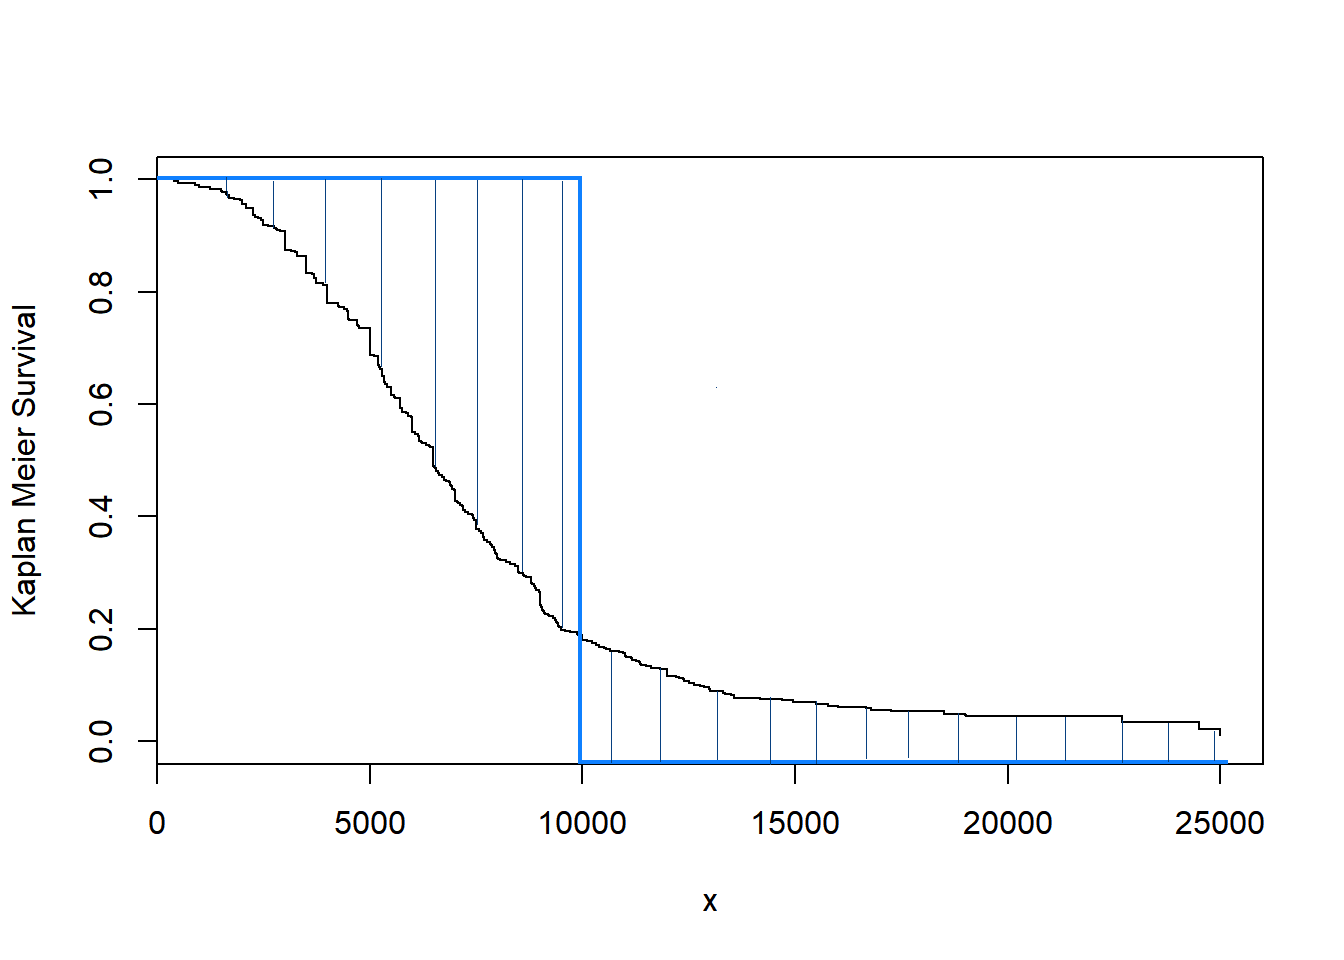
\includegraphics[width=.9\linewidth]{./Logos/survival2.png}
\caption{\label{fig:orgf7bccbc}
Survival function residual}
\end{figure}
  The light blue line corresponds to the ideal survival function and the area between the ideal and
  the actual survival, corresponds to the residual.
\end{block}

\begin{block}{Results}
The final model parametric obtained was compared to a model without covariates. This comparison
was made through the Brier score over all 18 machines. As mentioned before, the smaller the area of the
given Brier score closer the survival function is to that which is perfectly capable of telling
when the event will happen. As seen in the figure bellow, there was a significant improvement by using covariates.
\begin{figure}[htbp]
\centering
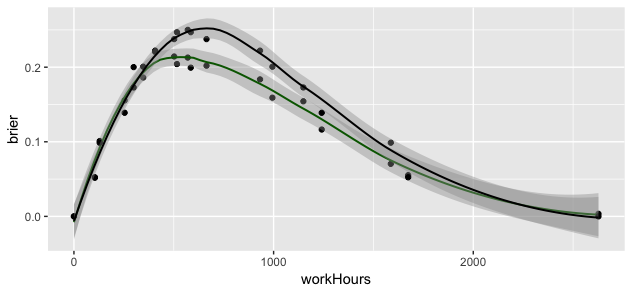
\includegraphics[width=.9\linewidth]{./Logos/finalbrier2.png}
\caption{\label{fig:orgfe2439b}
Comparison with the no covariate case}
\end{figure}
    The green line corresponds to the Brier using covariates and the black line to the no covariate case. 

    Despite this result, the final model is not suitable for production use. The main reason was due to the definition of a failure
    event not being clear. With the given data, it was not possible to distinguish between Instandsetzung and Instandhaltung events. 
    The repairs used for building the prediction model included routine maintenance,
    before the observation of the failure, hence, including bias in the model, since the mechanic could have 
    arbitrarily decided to repair the machine in any given time. 
\end{block}
\begin{block}{References}
\begin{enumerate}
\item Hisham M. Said and Tony Nicoletti. Telematics data-driven prognostics system for construction heavy equipment health monitoring and assessment. Construction Specialty Conference, 2015.
\item Hisham M. Said, Tony Nicoletti, and Peter Perez-Hernandez. Utilizing telematics data to support effective equipment fleet-management decisions: Utilization rate and hazard functions. Journal of Computing in Civil Engineering, 2015.
\end{enumerate}
\end{block}
\end{column}
\end{columns}
\end{frame}
\end{document}
